\chapter{Description of prototype functionality}\label{ch:descOfFunctionality}\vspace{-10mm}

With the modern teaching environment becoming evermore de-localised, we implemented a virtual whiteboard for remote-teaching with an emphasis on  mathematics.

\section{Lobby System}
The whiteboard, dubbed Mathboard, does not have any logins for simplicity. Instead, the host (the teacher), creates a 'room' which generates an associated 4-digit code. This can then be shared with potential viewers (the students) which allows them read-only access to the Mathboard.

\section{Standard Whiteboard Features}
As a whiteboard, the main feature is a pen. This can be used by the host to draw on the board in a variety of colours and thicknesses. The colours can be chosen either from a pre-defined pallet, a colours chooser (RGB or HSL) or a custom pallet to which colours can be saved.

The custom colour pallet can be saved and restored on any future Mathboard (provided they are on the same computer and browser, the storage is cookie-based).

All objects on the Mathboard can be edited as objects by the host - with resize, rotate, move and delete functions available.

\section{Mathematical Features}
The Mathboard is set apart from existing shared-whiteboards (of which there are many), by the integration of wolfram alpha. At the bottom of the hosts view is a text-query box into which almost anything can be typed from "Solve 2x+y\textasciicircum2=2 and x+y=0" to "Plot y=2x\textasciicircum3-9x\textasciicircum2+4x" and "What is the diameter of the earth?". The output of these queries is then inserted directly into the Mathboard. See figure 1 for the outputs of these particular queries.

Because of the sheer versatility of WolframAlpha (which is the engine behind Siri), this feature allows a plethora of mathematics to be computed directly into Mathboard.

\begin{figure}[!bp]
  \centering
  \begin{minipage}[b]{0.4\textwidth}
    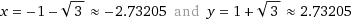
\includegraphics[width=\textwidth]{figures/fig1a.png}
    \caption{Output 1 for input Solve 2x+y\textasciicircum2=2 and x+y=0}
  \end{minipage}
  \hfill
  \begin{minipage}[b]{0.4\textwidth}
    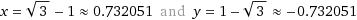
\includegraphics[width=\textwidth]{figures/fig1b.png}
    \caption{Output 2 for input Solve 2x+y\textasciicircum2=2 and x+y=0}
  \end{minipage}
\end{figure}

\begin{figure}[!bp]
  \centering
  \begin{minipage}[b]{0.4\textwidth}
    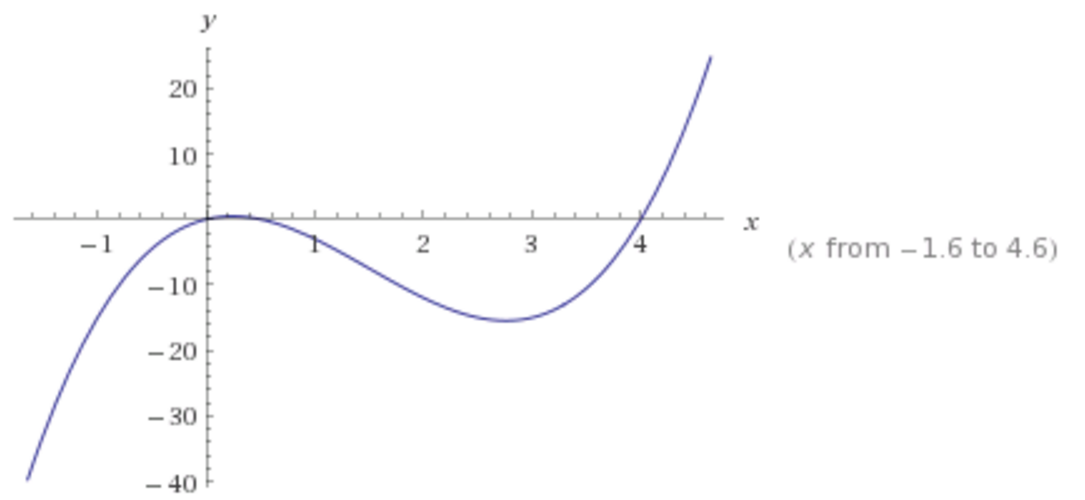
\includegraphics[width=\textwidth]{figures/fig2.png}
    \caption{Plot y=2x\textasciicircum3-9x\textasciicircum2+4x}
  \end{minipage}
  \hfill
  \begin{minipage}[b]{0.4\textwidth}
    
\includegraphics[width=0.5\textwidth]{figures/fig3.png}
    \caption{What is the diameter of the earth?}
  \end{minipage}
\end{figure}